\usepackage[pdftex]{graphicx}

\documentclass[a4paper,11pt]{uzreport}
\author{Mikołaj Mosoń
\\ 
\texttt{100324@stud.uz.zgora.pl} }
\group{33INF-SSI-SP/B} 
\type{p} 
\class{Systemy wbudowane}
\lab{Doniczka Hydroponiczna} 
\labnumber{ } 
\date{17/01/2021}
\supervisor{Piotr Mróz} 
\begin{document}
  \maketitle
  \clearpage


	\footnotesize
	\tableofcontents
	  \clearpage

\section{Wstęp}

Pierwszy raz o koncepcie stołów bezglebowych usłyszałem w grze RimWorld, na którą namówili mnie przyjaciele. Odkąd w nią zagrałem zastanawiałem się jak mógłbym samodzielnie zrealizować coś takiego. Zawsze miałem kłopoty z zadbaniem o rośliny więc pomysł samowystarczalnej doniczki wydał się idealny dla mnie.
Pierwszy raz próbowałem zrealizować taką doniczkę w marcu 2020. Utworzyłem wtedy koszyczki do utrzymywania rośln nad zbiornikiem z wodą. Postanowiłem ulepszyć dawny plan i zrealizować go w postaci projektu na systemy wbudowane.
\subsection{Cel czyli plan minimum}
Absolutnym minimum tego projektu jest uzyskanie doniczki która monitoruje warunki w jakich znajduje się roślina. Ponadto system musi sterować oświetleniem.
\section{Zasada działania}
\subsection{Schemat}
\begin{multicols}{2}
\begin{figure}[H]
    \centering
	     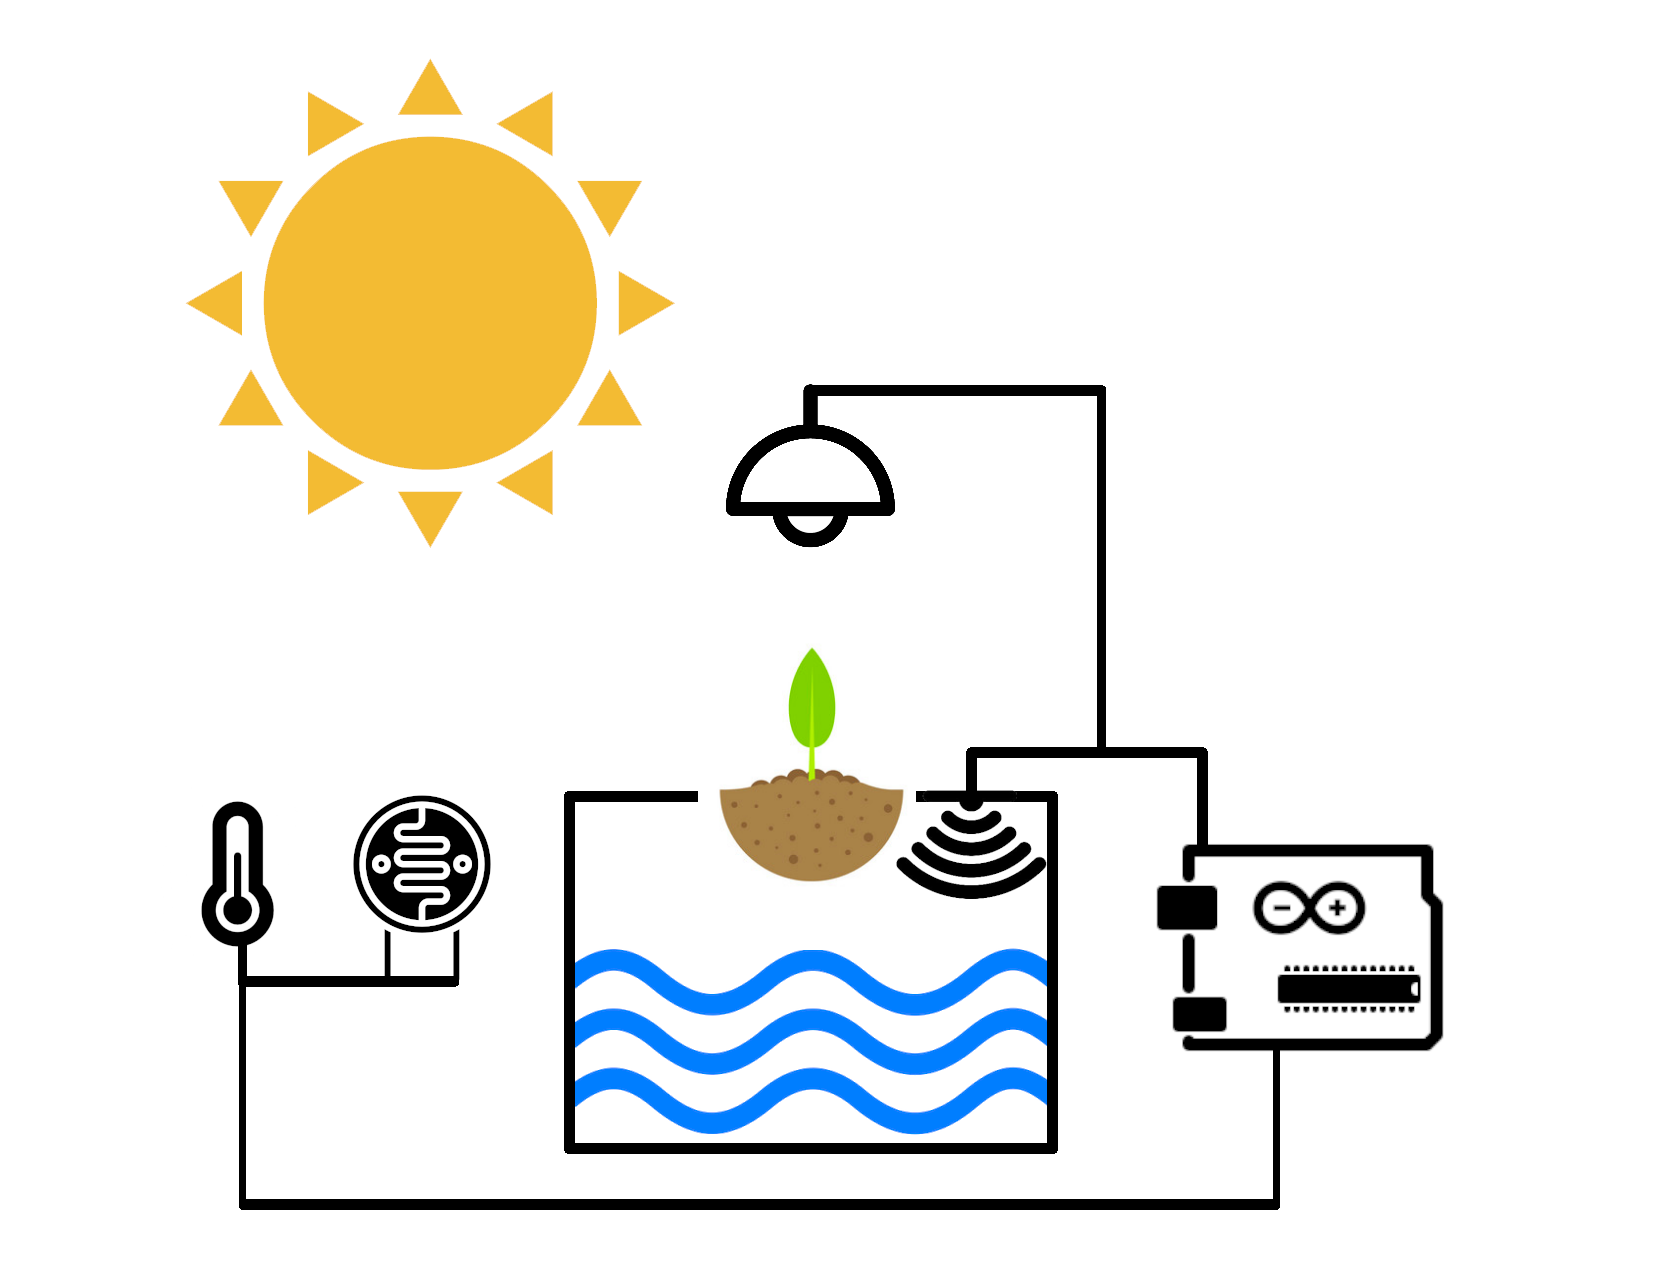
\includegraphics[width=\linewidth]{listings/doniczka_dzien.png}
    \caption{Działanie doniczki w trakcie dnia}
    \label{fig:my_label}
\end{figure}
\begin{figure}[H]
    \centering
		 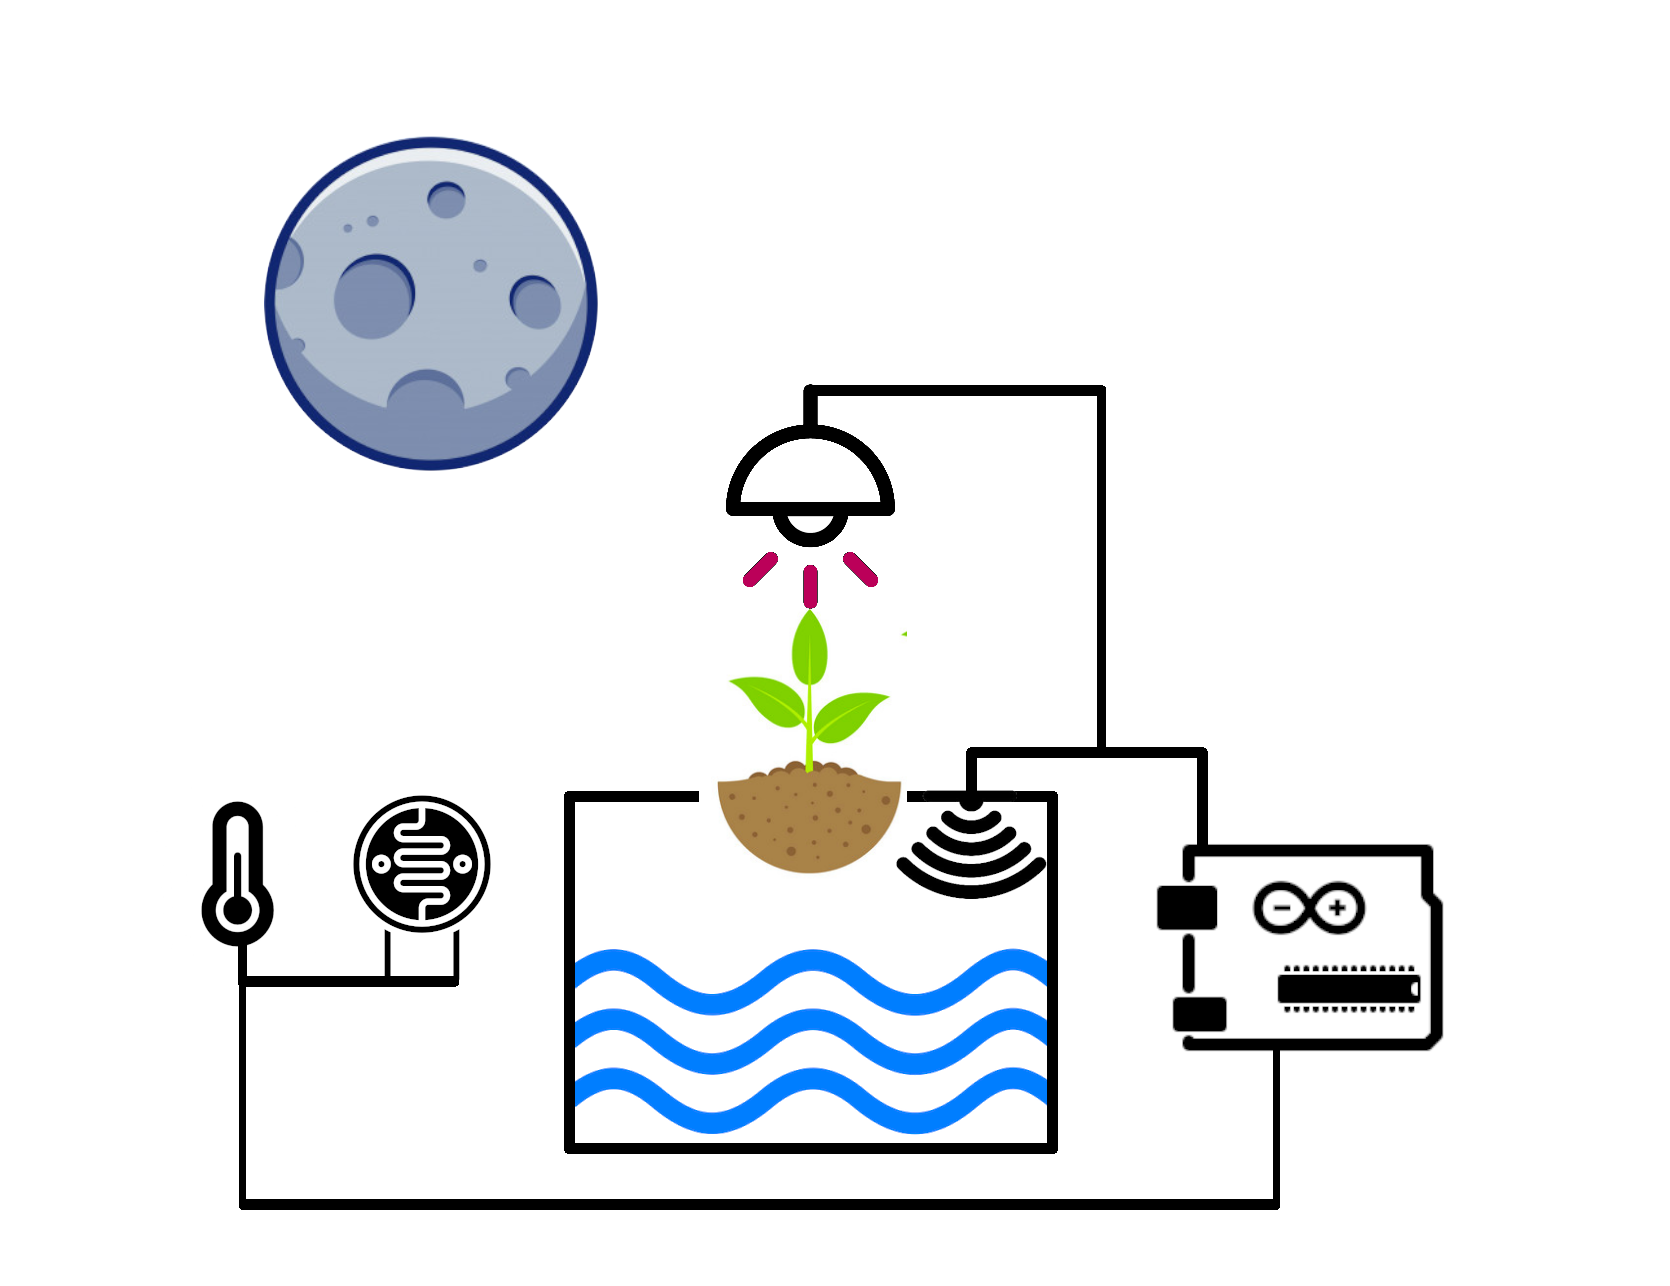
\includegraphics[width=\linewidth]{listings/doniczka_noc.png}
    \caption{Działanie doniczki w trakcie nocy}
    \label{fig:my_label}
\end{figure}
\end{multicols}
\subsection{Opis}
Doniczka będzie zawierała odpowiednie sensory do zbierania informacji.
\begin{itemize}
    \item fotorezystor
    \item czujnik poziomu wody
    \item czujnik temperatury
\end{itemize}
Na podstawie zebranych informacji z fotorezystora układ będzie ustalał aktualną porę dnia. Zadecyduje wtedy czy światło powinno być włączone czy nie. Na podstawie danych z czujnika temperatury system mógłby zdecydować czy zmienić ustawienia termostatu. Natomiast czujnik poziomu wody określiły czy należy dolać wody i włączyć pompę. Sam zbiornik z wodą zawierałby długoterminową pożywkę dla roślin. System pozwoliłby na zmaksymalizowanie wzrostu rośliny i zminimalizowanie wkładu użytkownika. To jest musiałby tylko dolewać wodę gdy zabraknie jej w rezerwuarze i dosypać pożywki gdy ta się skończy.
\clearpage
\subsection{Światło}
\begin{multicols}{2}
\begin{figure}[H]
    \centering
	     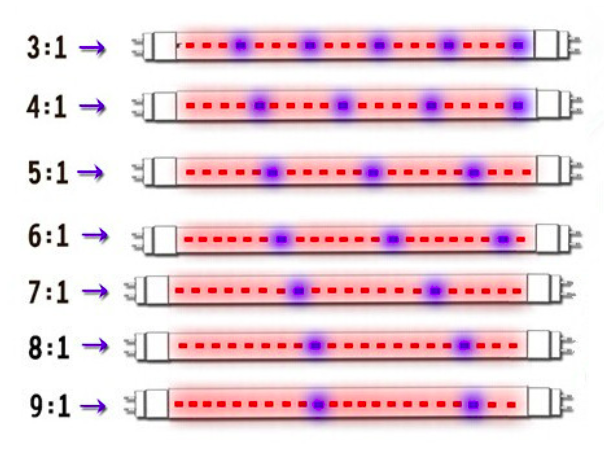
\includegraphics[width=.9\columnwidth,height=5cm]{listings/light.png}
    \caption{Proporcje świateł}
    \label{fig:my_label}
\end{figure}
	     \begin{text}
	         Do wzrostu roślinpotrzebny jest kolor czerwony i niebieski, zielony nie jest potrzebny jeżeli chce zastosować LED jako growing light.
                Według informacji które udało mi się znaleźć w internecie proporcje kolorów powinny być ustawiane tak jak na rysunku obok.\\
		         Gdzie pierwsze 3 wartości stosowane są dla roślin o dużych liściach takich jak np sałaty.\\
		         6:1 oraz 7:1 stosowane są dla sukulentów. \\
		         A ostatnie 2 wartości wspomagają rozwój korzeni.
	     \end{text}

\end{multicols}

\section{Model}
\subsection{Schemat}
\begin{figure}[!h]
    \centering
    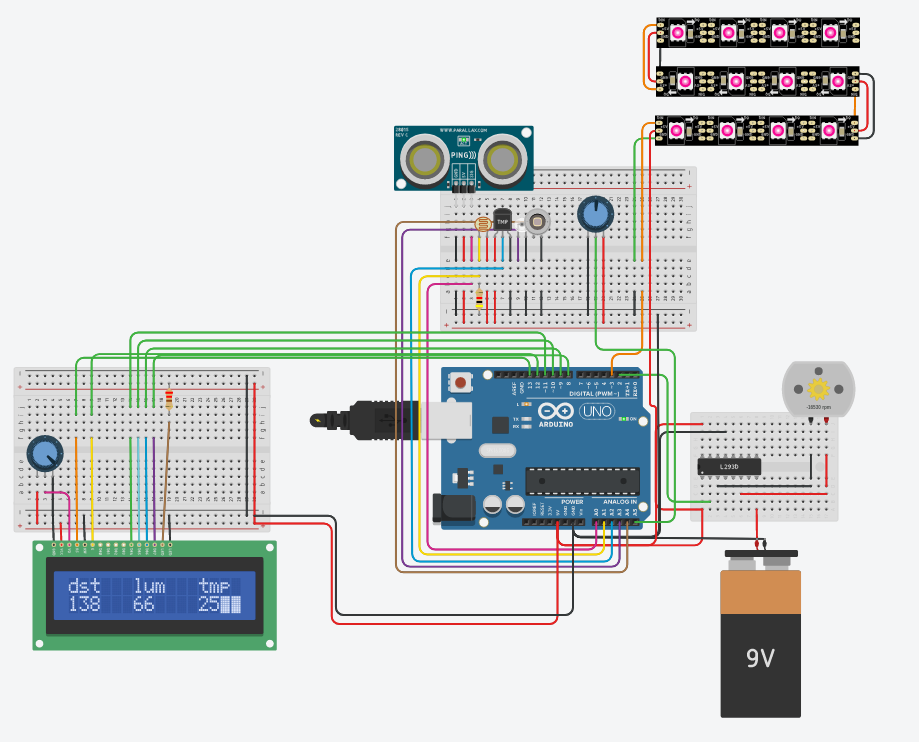
\includegraphics[width=\linewidth]{listings/zad1.png}
    \caption{Schemat wykonany w tinkercadzie}
    \label{fig:my_label}
\end{figure}
\clearpage
\subsection{Opis}
\begin{figure}
    \centering
      \href{https://www.tinkercad.com/things/2ZAZkGzNvPO-lab11}{https://www.tinkercad.com/things/2ZAZkGzNvPO-lab11}
    \captionsetup{labelformat=empty}
    \caption{Link do układu w tinkercadzie.}
    \label{fig:link}
\end{figure}
    \\
    Układ na początku zczytuje wartosci do tablicy values. Na jej podstawie sprawdzana jest najpierw ilość wody w rezerwuarze gdy czujnik zwraca wartość większą niż 10 cm włączana jest pompa, w przeciwnym razie pompa jest zatrzymywana. Klasa HydroSensors zwraca wartości światła w przedziale od 0 - 100. Sprawdzana jest wartość światła, gdy jest ona większa niż 50 zapalają się paski Neopixel. 
Proporcje świateł można ustalić za pomocą potencjometru. Wartości mapowane są od 1 do 9. Zastosowałem 3 paski po 4 diody. Oznacza to że każdy pasek zastosowany może być dla innej doniczki. Ilość diód ustalana jest na początku kodu.\\
Użytkownik jest informowany o wartościach czujników poprzez wyświetlacz LCD. Nie jest on w stanie wyświetlić w pełni wszystkich informacji na raz dlatego wyświetla tylko zaokrąglone wartości. Jeżeli użytkownik chce zobaczyć dokładniejsze wartości musi włączyć serial monitor dodatkowo serial monitor wyświetla proporcje czerwonych świateł do niebieskich.\\
\subsection{Kod}
\begin{center}
    \pythonCode{listings/zad1.txt}{Kod modelu}{lst:nested}
\end{center}
\subsection{Testowanie}
Układ sprawdzałem zmieniając ustalając na początku odpowiednią wartość światła. Wtedy zapalały się paski neopixel. Gdy powracałem do wartości startowych paski gasły tak jak powinny. Jak paski były zapalone sprawdzałem czy kolory się zmieniają gdy zmieniałem wartość potencjometru.
\section{Prototyp}
\subsection{Schemat}
\begin{figure}[!h]
    \centering
    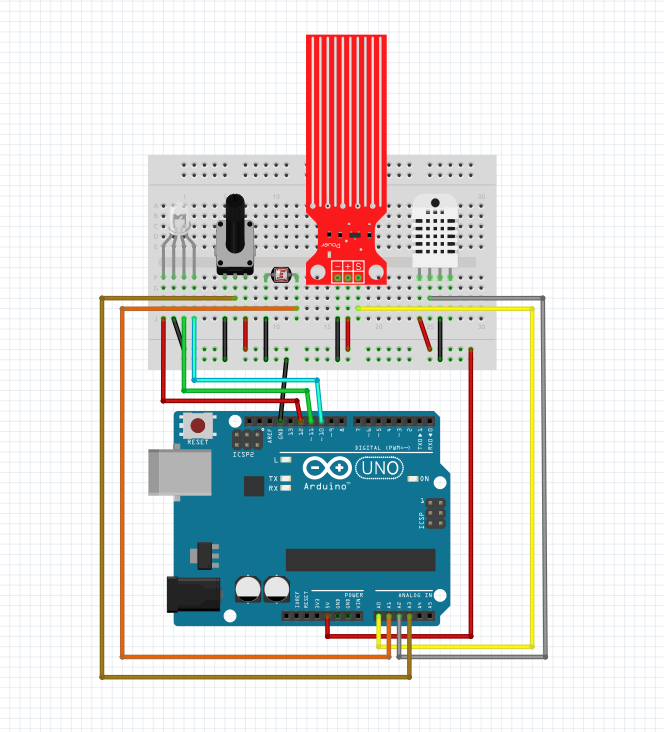
\includegraphics[height=10cm]{listings/uklad2.png}
    \caption{Schemat wykonany w programie fritzing. Ponieważ tinkercad nie zwierał odpowiednich komponentów. W schemacie nie uwzględniałem rezystorów ponieważ wszystkie komponenty które posiadam są w postaci złożonych modułów i mają je już wbudowane.}
    \label{fig:my_label}
\end{figure}
\subsection{Spis części}
\begin{itemize}
    \item Aduino UNO R3
    \item Fotorezystor
    \item Czujnik poziomu wody
    \item Dioda LED RGB
    \item Moduł DHT11 (czujnik temperatury i wilgoci)
    \item Potencjometr
\end{itemize}

\subsection{Opis}
Ze względu na to że model tworzyłem zanim kupiłem arduino różni się on od modelu. Zastosowałem inny czujnik temperatury ten w prototypie ma wbudowany czujnik wilgotności. Postanowiłem zastosować tylko fotorezystor do pomiaru światła. Uznałem ze względów praktycznych że dla pojedyńczej rośliny lepiej będzie nie stosować pompy. Poza tym niestety nie miałem tej części. Do pomiaru poziomu wody udało mi się uzyskać odpowiedni do tego czujnik, dlatego nie zastosowałem czujnika ultradźwiękowego. Jeżeli chodzi o światło nie posiadałem całęgo paska tylko pojedyńczą diode.
\subsection{Kod}
\begin{center}
    \pythonCode{listings/kod2.txt}{Kod prototypu}{lst:nested}
\end{center}
\subsection{Testowanie}
\subsubsection{Zbudowany układ}
\begin{multicols}{3}
\centering
	     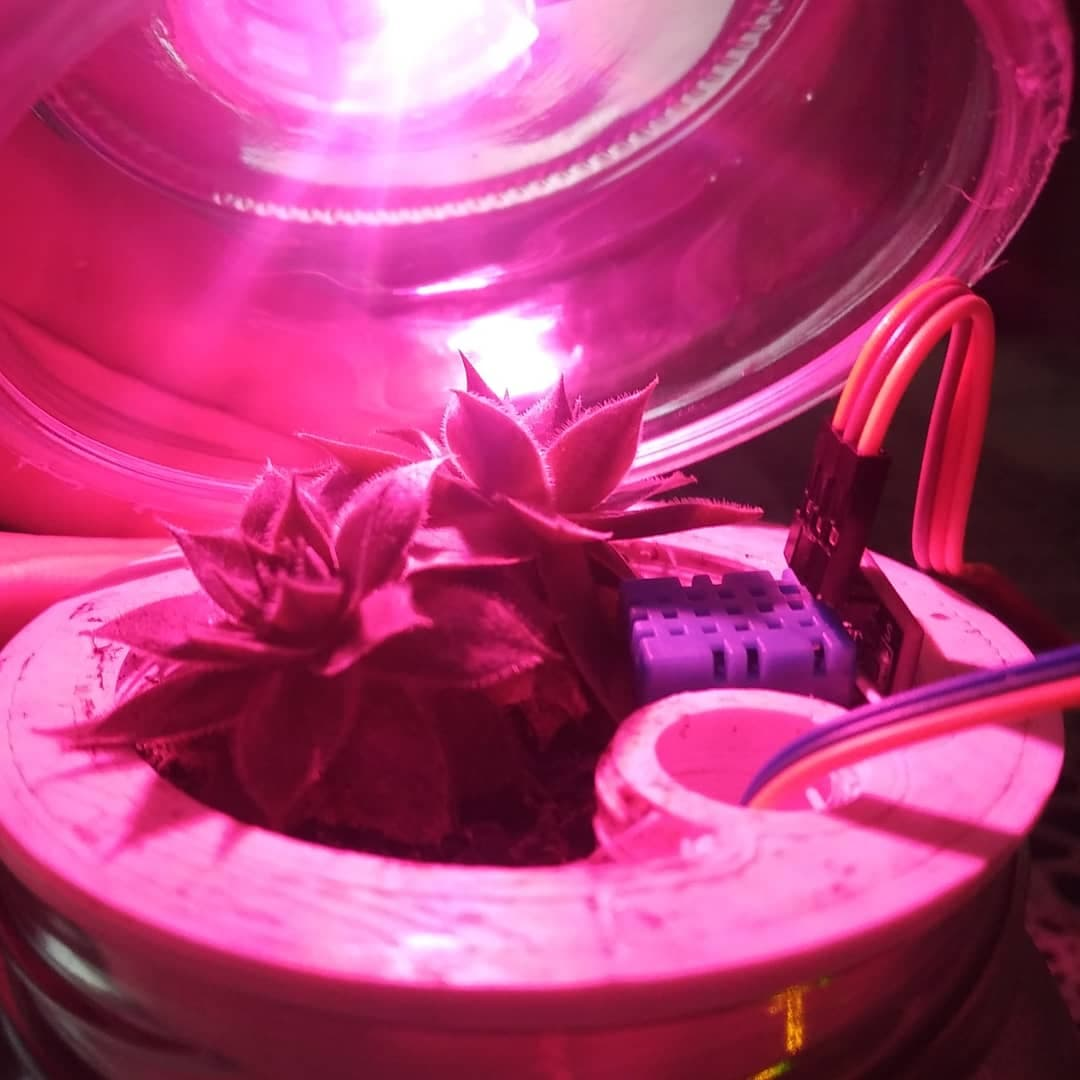
\includegraphics[width=.9\columnwidth,height=5cm,keepaspectratio]{listings/swiecisie.jpg}
		 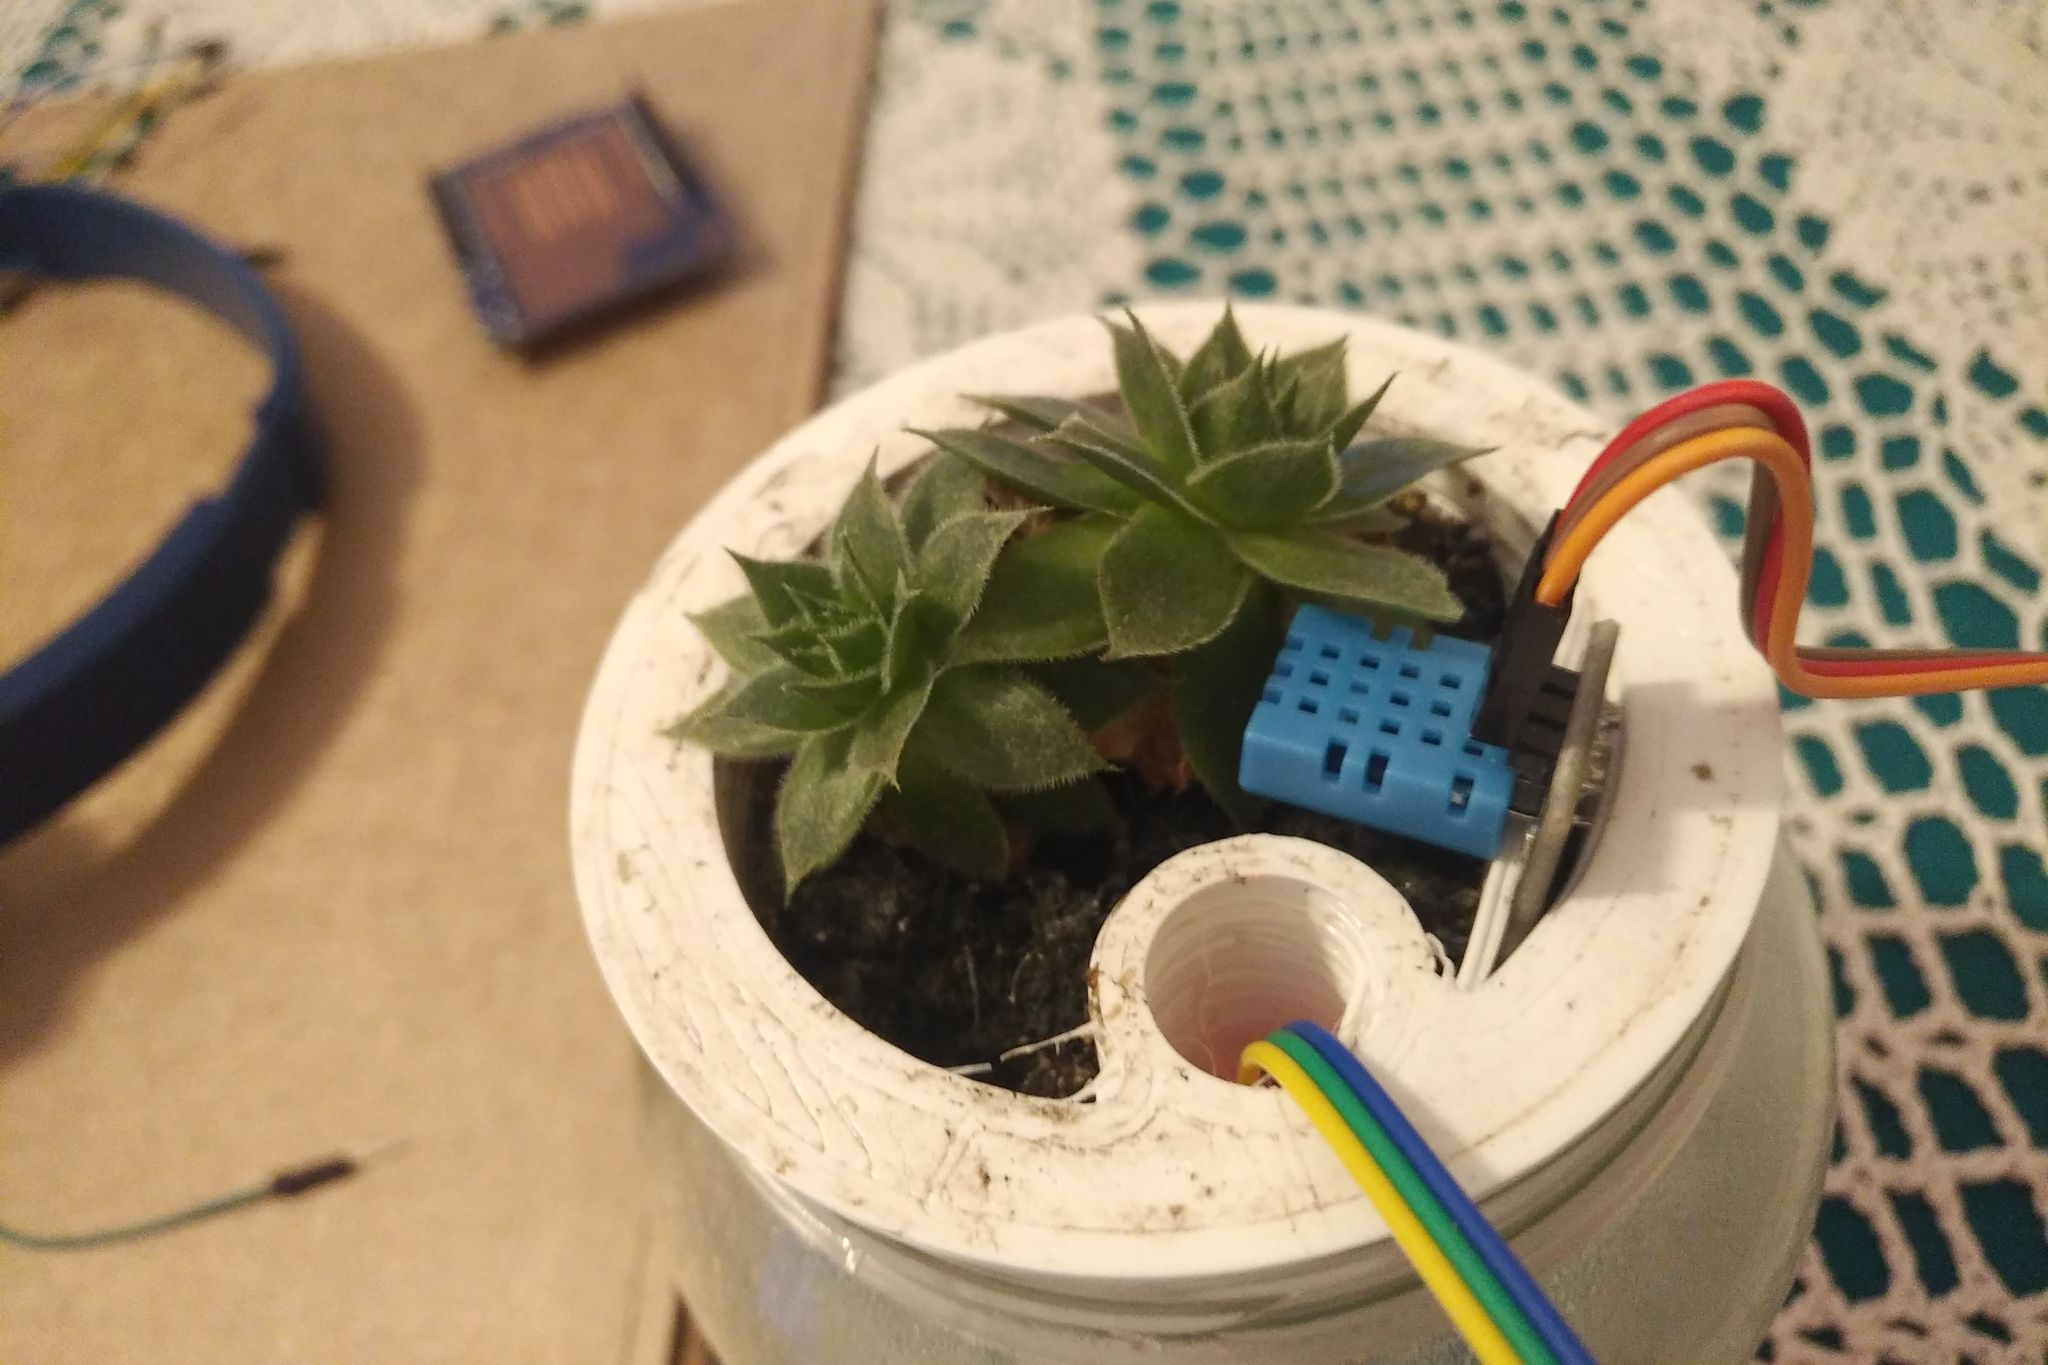
\includegraphics[width=.9\columnwidth,height=5cm,keepaspectratio]{listings/brakswiatla.jpg}
	     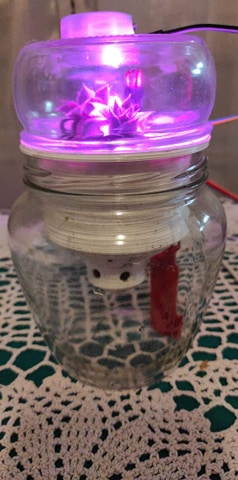
\includegraphics[width=.9\columnwidth,height=5cm,keepaspectratio]{listings/calosc.jpg}
		 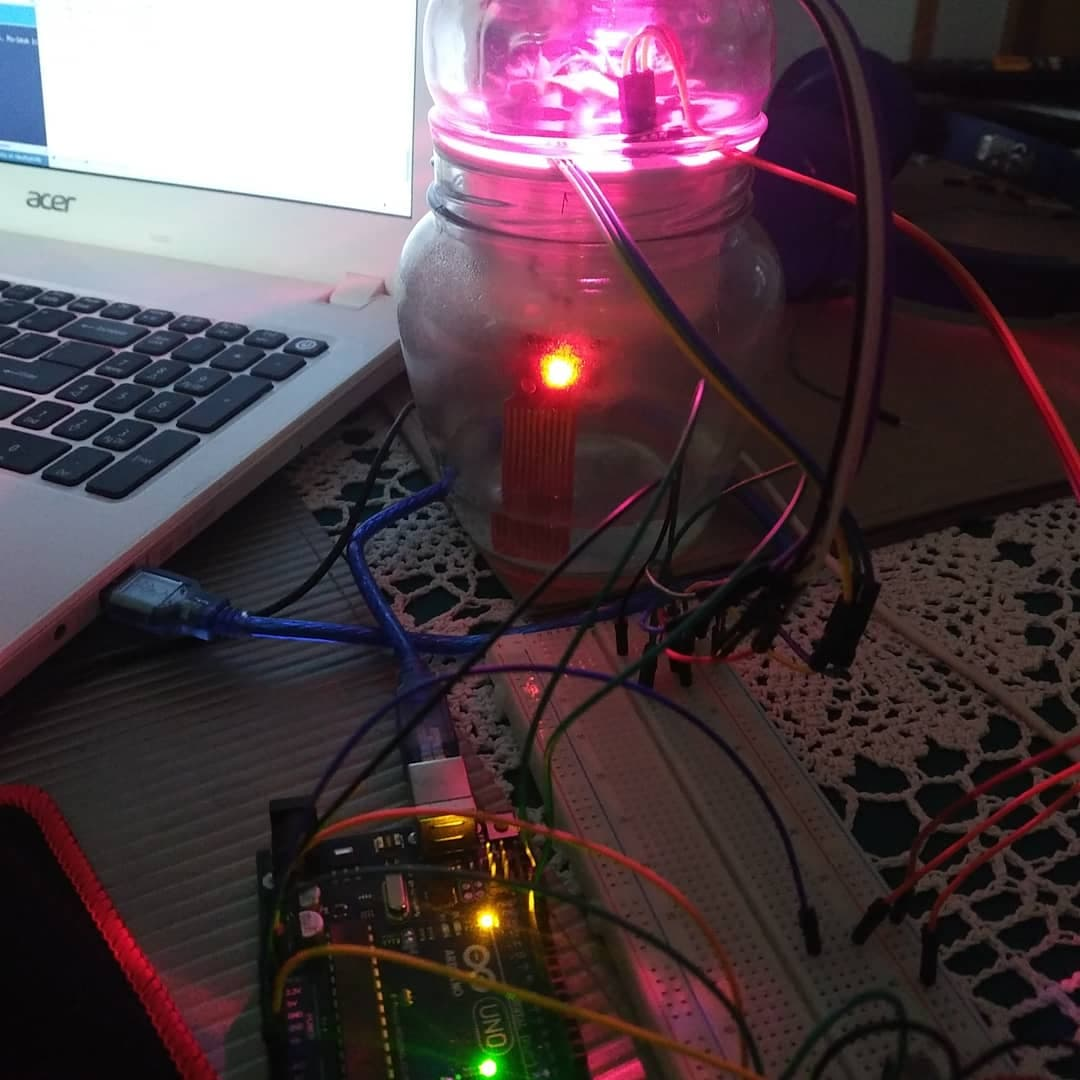
\includegraphics[width=.9\columnwidth,height=5cm,keepaspectratio]{listings/calosctest.jpg}
	     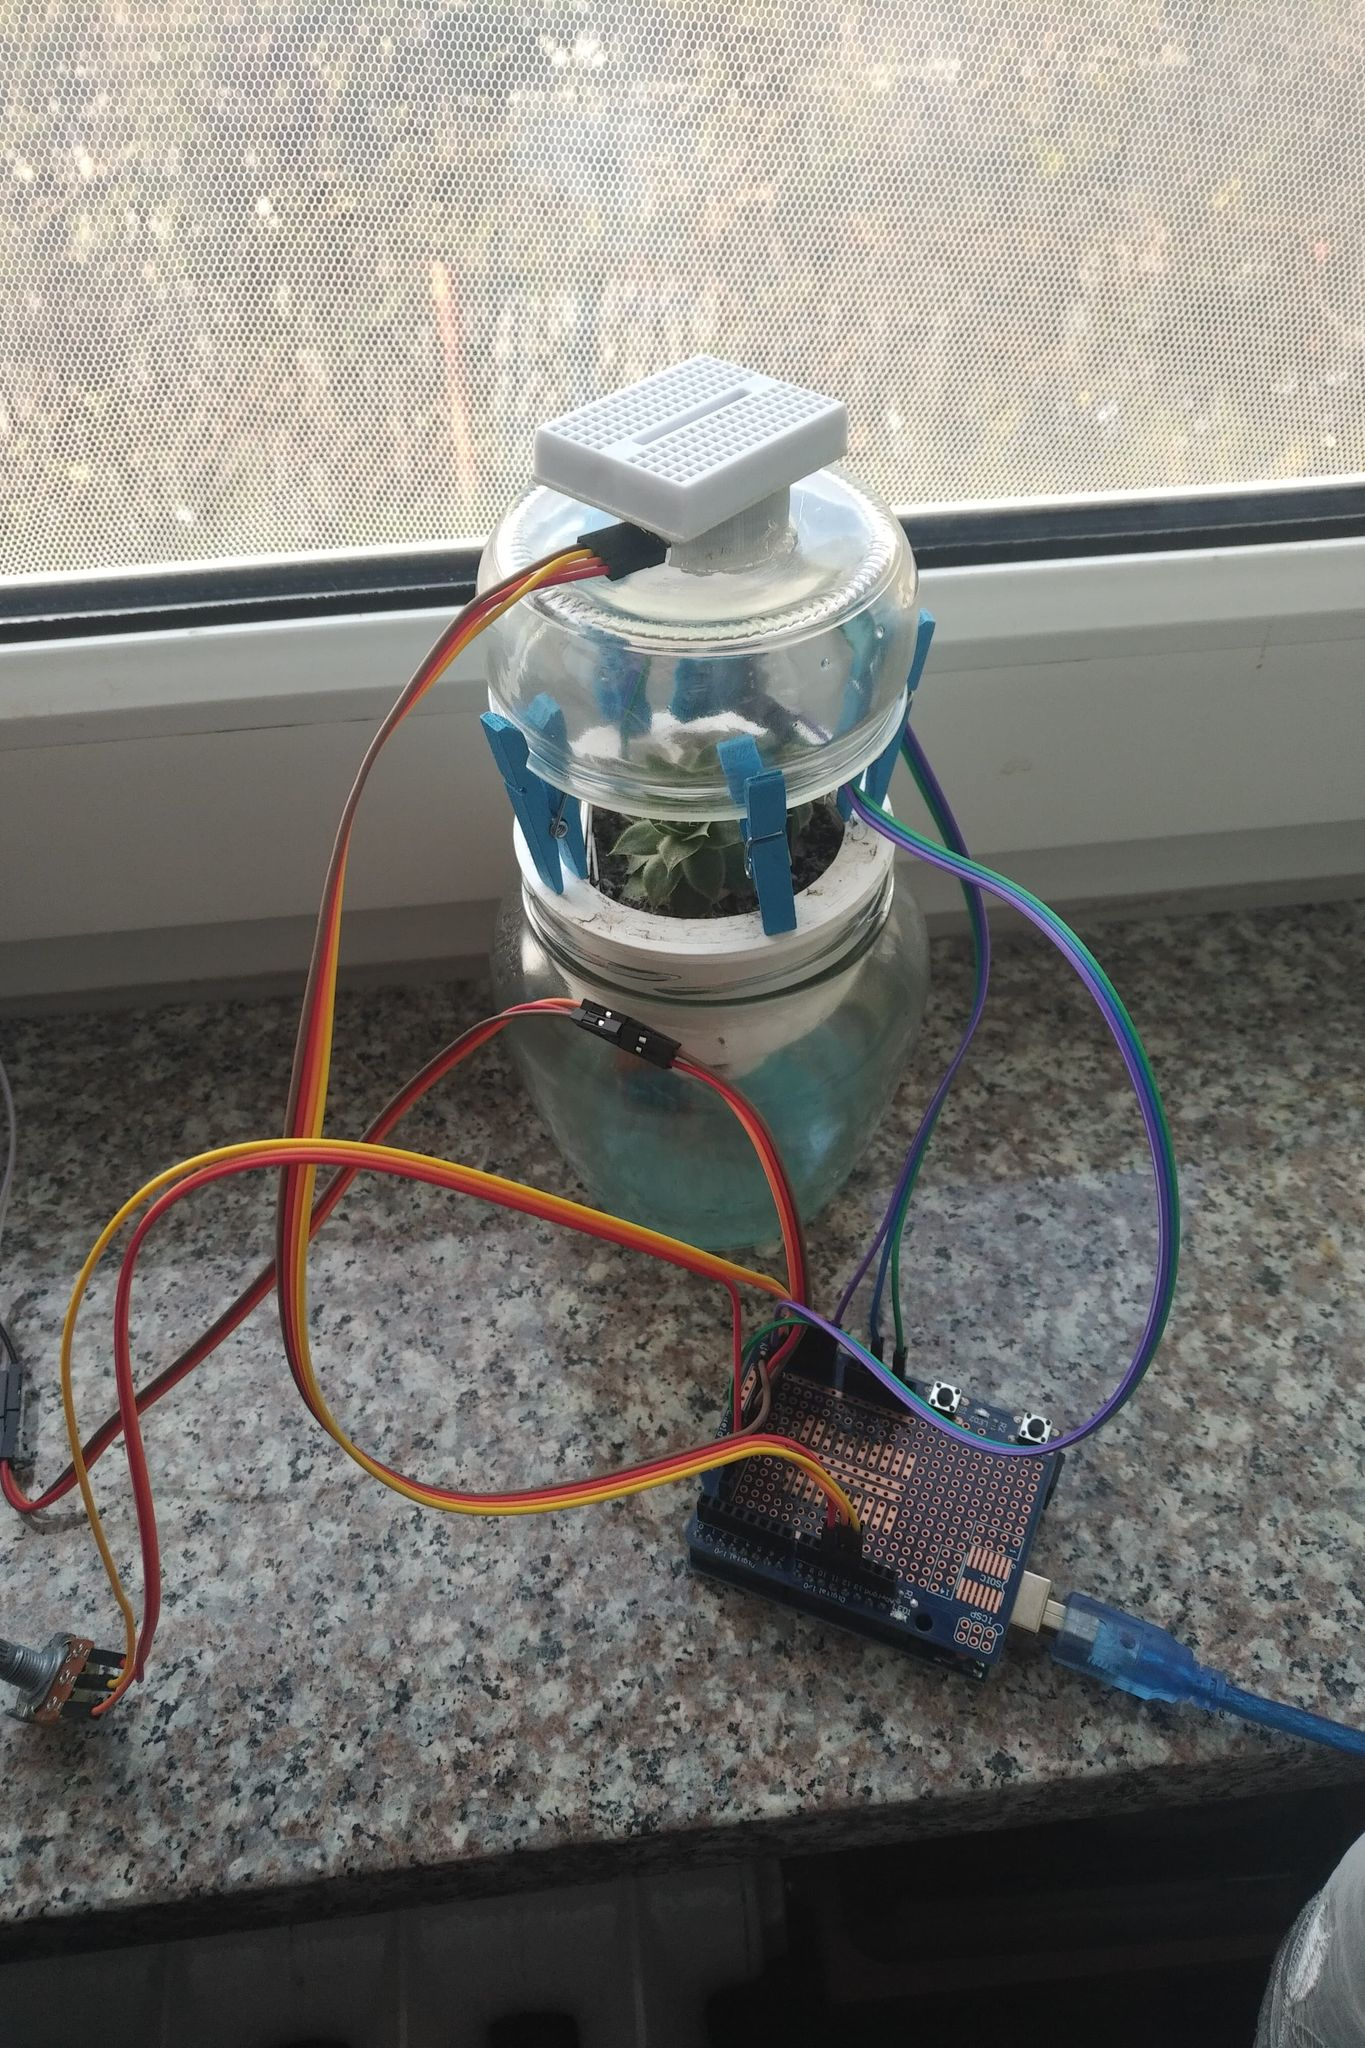
\includegraphics[width=.9\columnwidth,height=5cm,keepaspectratio]{listings/miejscetestowe.jpg}
		 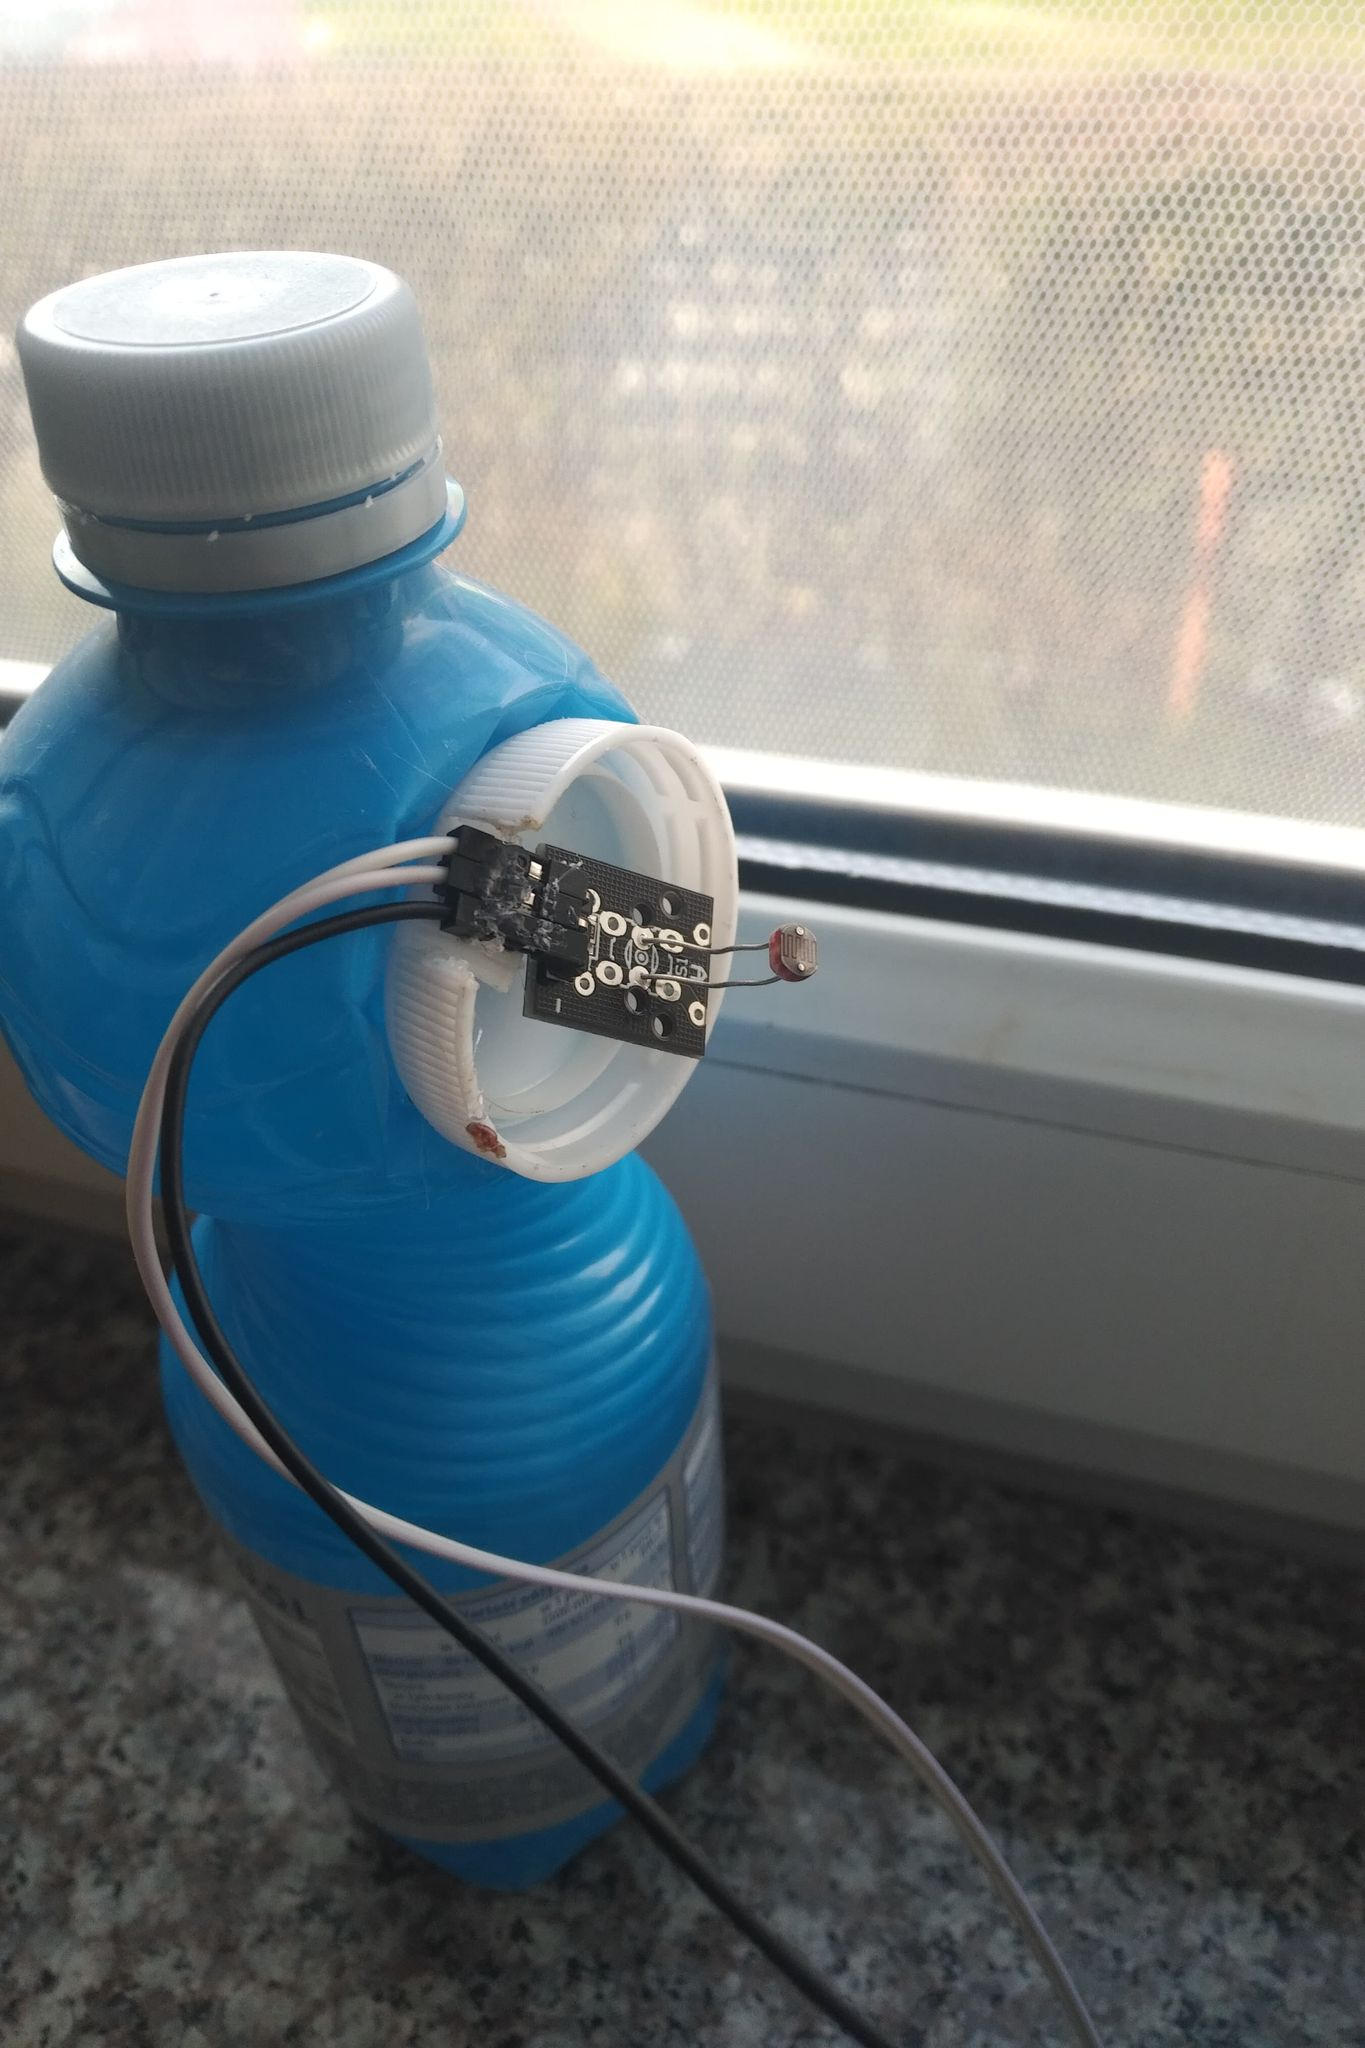
\includegraphics[width=.9\columnwidth,height=5cm,keepaspectratio]{listings/czujnikswiatla.jpg}
\end{multicols}
\subsubsection{Timelapse}
\begin{figure}[!h]
    \centering
      \href{https://www.youtube.com/watch?v=TiQmTjOGO_o}{https://www.youtube.com/watch?v=TiQmTjOGO_o}
    \captionsetup{labelformat=empty}
    \caption{Link prowadzi do video na youtubie pokazujacy timelapse z działania układu.}
    \label{fig:link}
\end{figure}
    Układ testowany był w godzinach 01:00 - 22:00, 13 stycznia. Niestety podczas testów 17 GB nagrania uległo uszkodzeniu ponieważ mój komputer sie zawiesił jedyne co udało mi się uratować to dane tektowe z godzin 01:00 - 13:00. Przedstawię te dane na wykresie poniżej. Ostatecznie udało mi się utworzyć time lapse ale pochodzi on z godzin 15:00 - 22:00.\\
    \begin{figure}[!h]
        \centering
        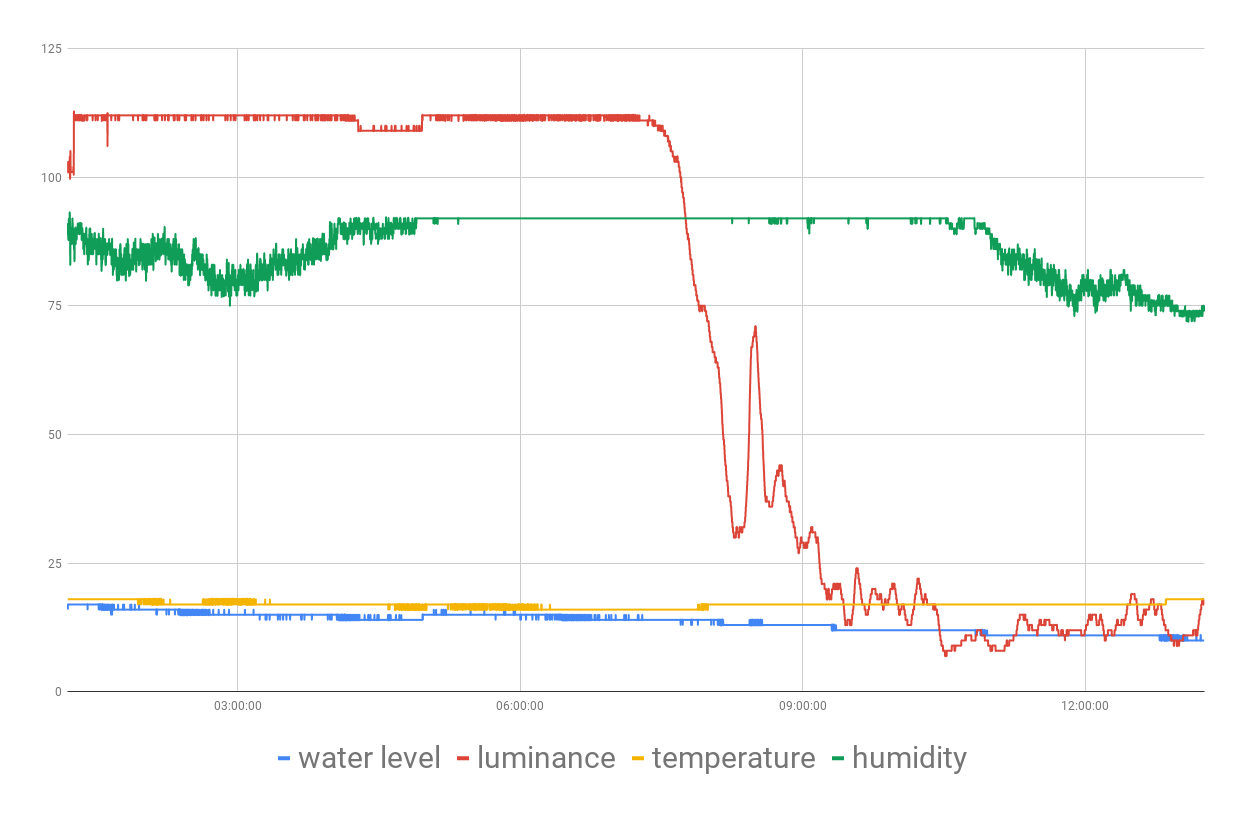
\includegraphics[width=\linewidth]{listings/chart .png}
        \caption{Dane pochodzące z godzin 01:00 - 13:00, 13 stycznia}
        \label{fig:my_label}
    \end{figure}
    Układ został umieszczony u mnie w pokoju. Około godziny 4 można zaobserwować nagły spadek poziomu światła oraz wzrost wilgotności w pokoju. Jest to spowodowane tym że o tej godzine kładłem się spać. Wilgotność wzrosła prawdopodobnie przez wydychane przeze mnie powietrze a wartość światła ponieważ zapalałem światło w pokoju. Jak widzimy okolo godziny 10 wartości wilgotności zaczeły spadać. Wtedy też skończyłem wykład i opuściłem pokój dlatego podejrzewam że moja obecność wpływała na wartości czujnika wilgotności. Niestety nie mam pojęcia co się stało w godzinach 07:00 - 08:00. Gdybym nie stracił nagrania byłbym w stanie odrazu stwierdzić. Wydaje mi się że ktoś mógł zapalić światło w pokoju obok i wpadło ono do mojego pokoju przez przeszklenie w drzwiach.
\subsubsection{Problemy}
        \begin{figure}[H]
        \centering
        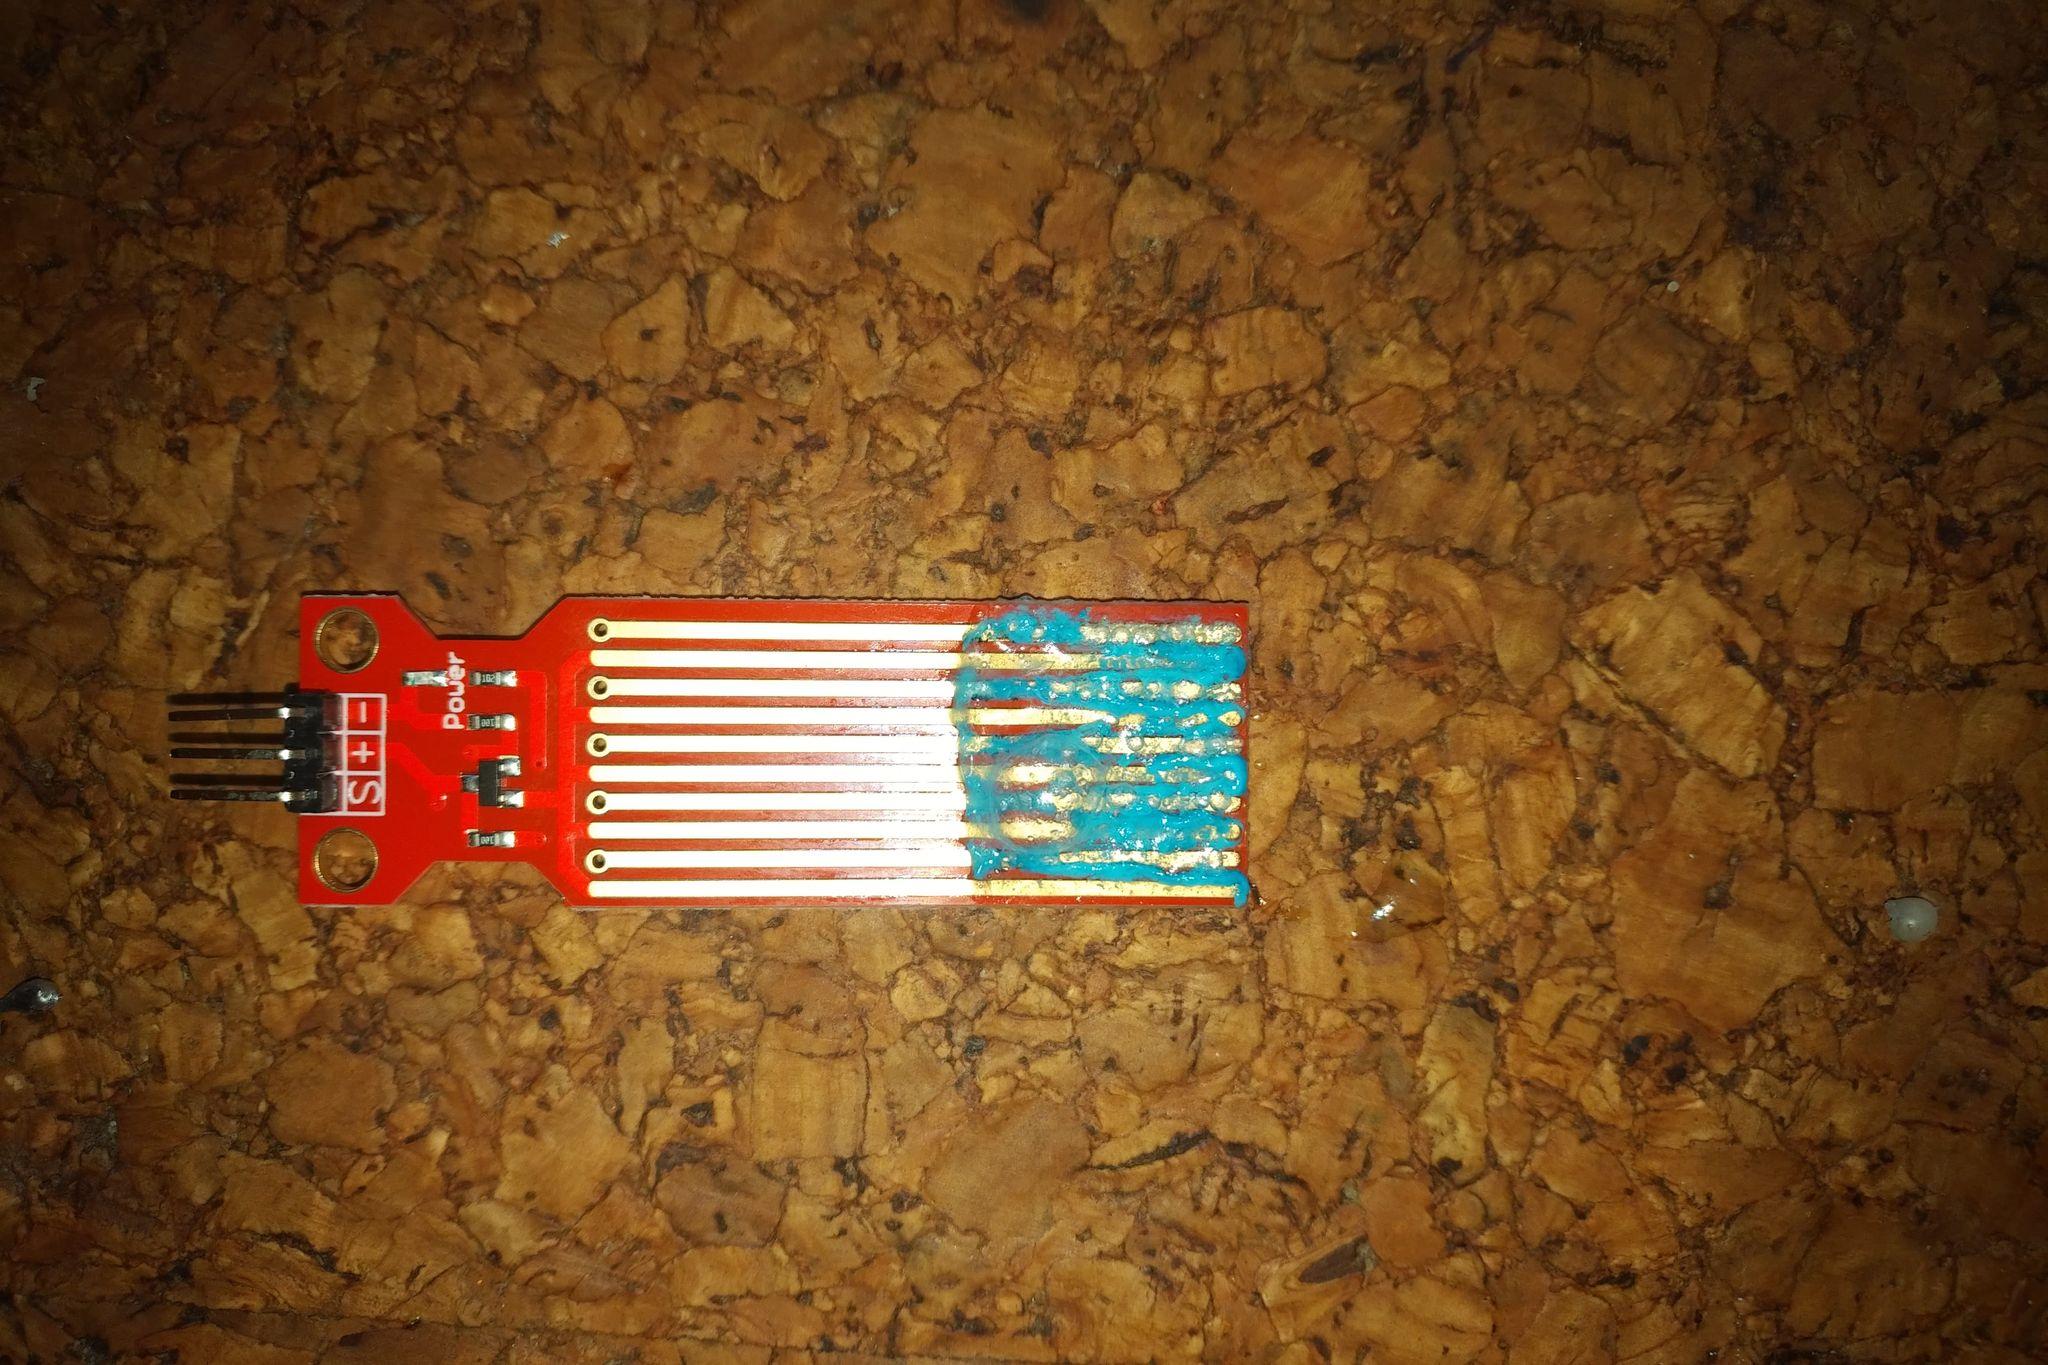
\includegraphics[width=\linewidth]{listings/sniedz1.jpg}
        \caption{Korozja na czujniku poziomu wody}
        \label{fig:my_label}
    \end{figure}
    Jeżeli chodzi o czujnik wody, możliwe że nie działał on prawidłowo. Podczas użytkowania pojawiła się na nim dość spora korozja. Udało mi się znaleźć informacje na temat tego czujnika i jednym z rozwiązań jest zmiejszenie natężenia oraz zwiększenie interwałów sprawdzania czujnika. Dlatego testowałem ten czujnik w 2 konfiguracjach. Zasilany 5V w interwałach 2 sekund, oraz 3.3V w interwalach 5 sekundowych.
    Oba przypadki kończyły się wspomnianą wcześniej korozją.\\

    Czujnik światła powinien wskazywać wartości od 0 do 100. Ale z jakiegoś powodu potrafi on wskazywać wartości powyżej 100. Nawet gdy mapuje go funkcją "map(((analogRead(photoResPin))), 0,1024, 0, 100)". Nie wiem czym jest to spowodowane niemniej jednak nie wpływa to na poprawność układu. Wynika to z tego że wartość graniczną dla zapalenia diody należy i tak wypracować metodą prób i błędów. 
    \subsection{Update}
    Z racji tego że ostatnie labolatorium na zajęciach z systemów wbudowanych było na temat Wielozadaniowości zaimplementowanie tej funkcji \ref{fig:update} nie było problemem. Projekt oddaje razem ze zrealizowaną wielozadaniowością.
    \begin{itemize}
        \item potencjometr sprawdzany jest w każdej pętli dzięki czemu niemal natychmistowo reaguje na zmiane proporcji światła,
        \item fotorezystor sprawdzany jest co 100ms dzięki czemu prawie odrazu zapala światło gdy jest to konieczne,
        \item DHT11 sprawdzane jest co 10 sekund, uważam że nie ma potrzeby sprawdzać go częściej jednak mimo wszystko musi byc sprawdzany minimalnie w interwale 2 sekund inaczej wyświetla błędy,
        \item czujnik wody sprawdzany jest co minutę, mam nadzieję że zmniejszy to korozję która pojawiła się na czujniku,
        \item Dane wyświetlane są w interwale 15 sekundowym
    \end{itemize}
    \pythonCode{update.txt}{Zmiany które dokonałem aby dodać wielozadaniowość}{}

\section{Wnioski}
Udało mi się zrealizować cel minimalny. To znaczy stworzyłem system do monitorowania warunków w których znajduje się roślina. Dodatkowo dodałem potencjometr który pozwala w trakcie działania układu zmieniać proporcje światła. Musiałem zrezygonować z niektórych funkcjonalności modlu, takich jak wyświetlacz i pompa wody. Wyświetlacz który posiadam niestety jest uszkodzony więc postanowiłem go pominąć, a małej pompy wodnej niestety nie posiadam.
\subsection{Plan rozwoju}
\subsubsection{Hardware}
\begin{itemize}
    \item  Wydaje mi się że oryginalny pomysł z sensorem ultradźwiękowym sprawdziłby się lepiej gdyby rezerwuar z wodą miał dla niego osobne miejsce.
    \item Zastąpić diody rgb żarówką led typu growing light. W tym momencie mam diode rgb i korzystam jedynie z kolorów czerwonego oraz niebieskiego, zielone światło jest niepotrzebne.
    \item Dodać przekaźnik SRD-05VDC-SL-C Songle pozwoli on sterować lampą i umożliwi zrealizowanie pkt powyżej.
    \item Dodać czujnik CO2
\end{itemize}
\subsubsection{Software}
\begin{itemize}
    \item \st{Umozliwic ukladowi wykonywanie wielu zadań jednoczesnie. W tym momencie uklad blokuje sie podczas wykonywania funkcji delay.}        \label{fig:update}

    \item Przebudowanie funkcji HydroSensor na klasę Sensors w której będzie można dynamicznie przypisywać jakie się chce czujniki.
    \item Dodać sterowanie za pomocą łącza serial port

\end{itemize}
\end{document}

